%%%% Dieses Werk ist unter der folgenden Lizenz lizenziert:
% Namensnennung-Keine kommerzielle Nutzung-Weitergabe unter gleichen Bedingungen 2.5 Schweiz
% http://creativecommons.org/licenses/by-nc-sa/2.5/ch/
% (C) 2008 Thorben Bochenek, Licia Huber, Remi Meier, Pascal Spörri
% (C) 2009 Pascal Spörri

\documentclass[a4paper,twocolumn]{article}
%\documentclass[a4paper]{article}

\usepackage{amsmath, amsthm, amssymb, amsfonts} 
\usepackage{german}
\usepackage[utf8]{inputenc}
\usepackage{multicol}  
%\usepackage{dsfont} 
\usepackage[rflt]{floatflt} % emerge -av floatflt
\usepackage{graphics}
\usepackage{epsfig}  

% ZuFa Template laden
\usepackage{tbabstract}
\columnsep24pt
\columnseprule0pt
\usepackage[font=small]{caption}

\title{Linalg\\HS08 ETHZ\\Zusammenfassung}
\author{Thorben Bochenek, Licia Huber, Remi Meier, Pascal Spörri}

\begin{document}
%\maketitle
%	Dieses Dokument ist unter der cc-by-nc-sa 2.5 ch (http://creativecommons.org/licenses/by-nc-sa/2.5/ch/) Lizenz lizenziert

%    \newpage
%\begin{multicols}{2}
\section{Matrizen}
	
	\vspace{-2mm}
	$$\begin{Large} A^{m \times n}      \end{Large} = 						
		\underbrace{
		\left( \begin{array}{cccc}
			a_{11} 	& a_{12} 	& \ldots 	& a_{1n} \\
			a_{21} 	& a_{ij} 	& \ldots 	& a_{2n} \\
			\vdots 	& \vdots 	& \ddots 	& \vdots \\
			a_{m1}	&a _{m2} 	&  \ldots    	& a_{mn} 
		\end{array} \right)  }_{n} \left. \begin{array}{c} \\ \\ \\ \\ \\ \end{array} \hspace{-5mm} \right\rbrace  m
	$$
		
	\begin{feig}[Mögliche Eigenschaften von Matrizen]
		\begin{desc_compact}
			\item[symmetrisch] $A = A^{T}$ ($\Rightarrow m = n$)
			\item[hermitesch] $A = A^{H}$, $A$ gleich ihrer konjugiert komplexen Transponierten
			\item[positiv definit] $\forall x: x^H Ax > 0$ ($x \neq 0$ $A$ symmetrisch/hermitsch)\\
				Matrix positiv definit $\Leftrightarrow \exists$ Choleskyzerlegung
			\item[positiv semidefinit] $x^H A x \geqslant 0$ ($x$ darf $0$ sein)
			\item[orthogonal (unitär $\mathbb{C}$)] $A \cdot A^{T} = I \longrightarrow A^{-1} = A^T$
			\item[$A$, $B$ kommutieren] $A \cdot B=B \cdot A$
			
		\end{desc_compact}
			\vspace{-3mm}
	\end{feig}
	
	\subsubsection{Die Transponierte einer Matrix}
		\begin{fdef}[Normalfall $A^T$]
			Zeilen und Spalten vertauschen:
			\begin{align*}
				\left( \begin{array}{ccc}
				        1 & 2 & 3\\
				        4 & 5 & 6
				       \end{array} \right)^T = 
				       \left(
				       		\begin{array}{cc}
				       			1 & 4\\
				       			2 & 5\\
				       			3 & 6
				       		\end{array} \right)
			\end{align*}
		\end{fdef}
		\begin{fdef}[$A$ besitzt komplexe Einträge]
			Hat $A$ komplexe Einträge s definiert man $B=A^H$ als die $n\times m$ Matrix $B$ mit $b_{ij} = \overline{a_{ji}}$  ($\overline{\alpha + i \beta} = \alpha - i \beta$)
			\begin{align*}
				\left( \begin{array}{cc}
				        2+i & 3-i\\
				        1+i & 1-i 
				       \end{array} \right)^H =
				       \left( \begin{array}{cc}
				               2-i & 1-i\\
				               3+i & 1+1
				              \end{array} \right)
			\end{align*}

		\end{fdef}

		
	\subsection{Lineare Gleichungssyteme (LGS)}
		
		$A \cdot x = b$ \hspace{8mm}
		Lösung: $x = A^{-1} \cdot b$ $\\$
		$\rightarrow$ $m$ Gleichungen, $n$ Unbekannte
		
		\begin{fdef}[Rang]
			Anzahl der linear unabhängigen Vektoren der Matrix (entspricht Anz. Zeilen $\ne 0$ der Matrix in Stufenform)
		\end{fdef}
			alle Vektoren unabhängig $\Rightarrow$ Rang vollständig, Matrix \textbf{regulär}, $m = n$\\
			sonst Matrix \textbf{singulär}
		
		\begin{feig}[homogen]
			$Ax = 0$ (rechte Seite $= 0$)
		\end{feig}
		
		\begin{fmerke}[Lösungen von LGS]
			\begin{description}
				\item $\left. \begin{array}{c}$
						$\mathbf{Ax=b} \\$ $\textit{hat genau}$ $\\$ $\textit{eine L"osung}$
					$\end{array} \right\}$
					$\Leftrightarrow \left\{ \begin{array}{c}$
					$r=n=m$ oder $\\$
						$\left\{ \begin{array}{c}$
							$r=n<m$ und $\\$
							$c_{r=1}=\cdots=c_m=0$ 
						$\end{array} \right\}$
					$\end{array} \right.$,
					
				\item $\left. \begin{array}{c}$
						$\mathbf{Ax=b} \\$ $\textit{hat f"ur jedes}$ $\mathbf{b}\\$ $\textit{(mind.) eine L"osung}$
					$\end{array} \right\}$
					$\Leftrightarrow$
					$r=m$,
					
			\item $\left. \begin{array}{c}$
						$\mathbf{Ax=b} \\$ $\textit{hat f"ur jedes}$ $\mathbf{b} \\$ $\textit{genau eine L"osung}$
					$\end{array} \right\}$
					$\Leftrightarrow$
					$r=m=n$,
			\end{description}
		\end{fmerke}


		
	\subsection{Rechnen mit Matrizen}
		
		\begin{fdef}[Multiplikation]
			Matrixdimensionen: $m \times n \cdot n \times p = m \times p$
		\end{fdef}
		
		\begin{falgo}[Multiplkationsalgorithmus]
			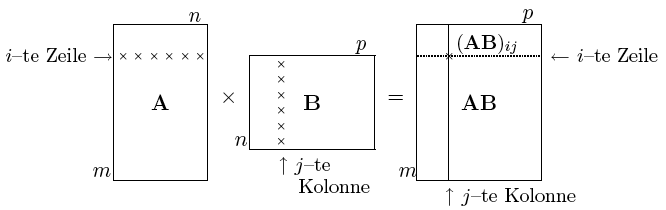
\includegraphics[width=\textwidth]{matrix_multiplikation}
			Man multipliziert alle $A_{1,j}$ mit den dazugehörign $B_{i,1}$ und addiert jeweils die Resultate $\Rightarrow$ ergibt 
			das erste Element der Multiplikationsmatrix, Schritt wiederholen für alle $A_{i,j}$ und $B_{i,j}$
		\end{falgo}
		
		$(ab)_{ij}=\sum_{k=1}^n a_{ik}\cdot b_{kj}$\\[1mm]
			$A \cdot B^T = \sum^n_{j = 1} a_j b_j^T$ oder $(A^T B)_{ij} = a_i^T b_j$ wobei $a_j$ der $j$-te Kolonnenvektor von $A$ ist
			
		\begin{fregeln}[Rechnen mit Matrizen]
			\vspace{-5mm}
			\begin{multicols}{2}
			$(\alpha + \beta)A = \alpha A + \beta A$\\
			$A + B = B + A$\\
			$A(B + C) = (AB) + (AC)$\\
			$(A + B)^H = A^H + B^H$\\
			$(AB)^H = B^H A^H$\\
			$AB \ne BA \; \text{ \small im Allgemeinen}$\\\small wenn doch: $AB$ kommutieren\\
			$(AB)^{-1} = B^{-1} \cdot A^{-1}$\\
			$(\alpha A)^{-1} = \alpha^{-1} \cdot A^{-1}$\\
			$(A^{-1})^H = (A^H)^{-1}$
			\end{multicols}
			\vspace{-3mm}
	\end{fregeln}
	\subsection{Inverse der Matrix}
		\begin{fdef}[Inverse Matrix]
			$A^{-1} := $ Inverse von $A$ \hspace{4mm} $A \cdot A^{-1} = I = A^{-1} \cdot A$
		\end{fdef}
			\vspace{-2.5mm}
			$A$ invertierbar $\leftrightarrow$ $A$ regulär
		
		\begin{fdef}[Rechenregeln]
			\begin{align*}
				(A^{-1}){-1} = A \qquad (AB)^{-1} = B^{-1}A^{-1} \qquad (A^H)^{-1} = (A^{-1})^H
			\end{align*}

		\end{fdef}

		\begin{falgo}[Gauss-Jordan-Algorithmus]
			\textbf{Anwendung: }Berechnung der Inversen und Lösen von linearen Gleichungssystemen\\[1mm]
			\textit{Inverse}: Marix neben Einheitsmatrix. Umwandeln von A in Einheitsmatrix, wobei dieselben Operationen auf I angewendet werden. Verändertes I ist $A^{-1}$
			\begin{align*}
			\underbrace{
				\left( \begin{array}{ccc}
					a_{11} 	& \ldots 	& a_{1n} \\
					\vdots 	& \ddots 	& \vdots \\
					a_{m1} 	& \ldots  	& a_{mn}
				\end{array} \right)
			}_A
			\quad
			\underbrace{
				\left( \begin{array}{ccc}
					1	 	& \ldots 	& 0		 \\
					\vdots 	& \ddots 	& \vdots \\
					0	 	&  \ldots  	& 1
				\end{array} \right)
			}_I \\
				\vdots
			\underbrace{
				\left( \begin{array}{ccc}
					1	 	& \ldots 	& 0		 \\
					\vdots 	& \ddots 	& \vdots \\
					0	 	&  \ldots  	& 1
				\end{array} \right)
			}_{A \rightarrow I}
			\quad
			\underbrace{
				\left( \begin{array}{ccc}
					b_{11} 	& \ldots 	& b_{1n} \\
					\vdots 	& \ddots 	& \vdots \\
					b_{m1} 	& \ldots  	& b_{mn}
				\end{array} \right)
			}_{I \rightarrow A^{-1}}
			\end{align*}
	\end{falgo}	
	\begin{falgo}[Inverse allgemeiner 2x2 Matrizen]
			$\bigtriangleup$-Matrizen
			\begin{align*}
				A= \left(
					\begin{array}{cc}
						a_{11} & a_{12} \\
						0	   & a_{22}
					\end{array}
					\right) \text{ wenn $a_{11} \neq 0$, $a_{22} \neq 0$, dann } \\
				A^{-1}= \left(
					\begin{array}{cc}
						\frac{1}{a_{11}} & - \frac{a_{12}}{a_{11}a_{22}} \\
						0				 &   \frac{1}{a_{12}}
					\end{array} \right) 
			\end{align*} 
			Normalfall
			\begin{align*}
				A = \left( 
					\begin{array}{cc}
						a_{11} & a_{12} \\
						a_{21} & a_{22}
					\end{array} \right)
						\text{ wenn $a_{11}a_{22} - a_{12}a_{21} \neq 0$ } \\
				A^{-1} = \frac{1}{a_{11}a_{22} - a_{12}a_{21}} \cdot 
					\left( 
						\begin{array}{cc}
							a_{22} & -a_{12} \\
							-a_{21} & a_{11}
						\end{array} 
					\right)
			\end{align*}
		\end{falgo}
		
		\begin{falgo}[Geschlossene Form]
			
			\begin{align*}
				A^{-1} = \dfrac{1}{\det(A)} \cdot C^T \text{ wobei: }  C_{ij} = (-1)^{i+1} \det(A_{ij})
			\end{align*}

		\end{falgo}



			
\subsection{Normen}
		\begin{fdef}[Norm]
			$1$-Norm (Manhattan Norm)
			\begin{align*}
				||x||_1=  |x_1| + |x_2| + \hdots + |x_n|
			\end{align*}
			$2$-Norm (Euklidische Norm / Standardnorm)
			\begin{align*}
				||x||_2= \sqrt{\langle x,x \rangle} = \sqrt{x^H\cdot x} = \sqrt{\sum_{i=1}^{n}|x_i|^2} 	
			\end{align*}
			$p$-Norm
			\begin{align*}
				||x||_p= \left( |x_1|^p + |x_2|^p + \hdots + |x_n|^p \right) ^{\frac{1}{p}} 
			\end{align*}

			$\infty$-Norm
			\begin{align*}
				||x||_{\infty} = \max ( |x_1|, |x_2|, \hdots, |x_n|)
			\end{align*}

		\end{fdef}
	
		\begin{feig}[Eigenschaften der Norm]
			Positiv definit
				$
					||x|| \ge 0 \\
					\langle x, x \rangle = 0 \Rightarrow x = 0
				$\\
			Symmetrisch\\
				$
					\langle x , y \rangle = \langle y, x \rangle
				$\\
			Linear\\
				$
					\langle x, y + z \rangle = \langle x, y \rangle + \langle x, z\rangle \\
					\langle x, \alpha y \rangle = \alpha \langle x, y \rangle
				$
		\end{feig}

		\begin{fmerke}
			\textbf{Schwarz'sche Ungleichung}\\[.5mm]
				$|\langle x,y \rangle| \le ||x|| \cdot ||y||$\\[2.5mm]
			\textbf{Dreiecksungleichung}\\[.5mm]
				$||x \pm y|| \le ||x|| \cdot ||y||$\\[-2mm]
		\end{fmerke}
		
	\subsection{Skalarprodukt}
	
		\begin{fdef}[Skalarprodukt, inneres Produkt]
			$\langle x,y \rangle = x^H y$
		\end{fdef}
		
		\begin{feig}[Eigenschaften SP]
			$\langle x,y \rangle = \overline{\langle y,x \rangle}$ \hspace{6mm}
			$\langle x,x \rangle \ge 0$ \\
			$\langle x,ay+z \rangle = a\langle x,y \rangle+ \langle x,z \rangle$\\
			$\rightarrow \langle ax+z,y \rangle = \overline{a} \langle x,y \rangle +\langle z,y \rangle$\\
		\end{feig}
			
		\begin{fmerke}[Winkel zwischen zwei Vektoren]
			$\langle x,y \rangle = ||x|| \cdot ||y|| \cdot \cos(\alpha) \quad $ wobei $\alpha = \measuredangle (x, y)$\\
			$\langle x,y \rangle = 0 \leftrightarrow x \perp y$ 
		\end{fmerke}
		
		\begin{fmerke}[Winkel an einem Punkt]
% 			\begin{multicols}{2}
				Der Winkel zwischen $\sphericalangle AEB$ ist definiert als der Winkel zwischen $v_1$ und $v_2$ wobei gilt:
				\begin{align*}
					v_1 = A-E \qquad v_2 = B-E
				\end{align*}
% 				\begin{figure}[htp]
					
					\begin{center}
						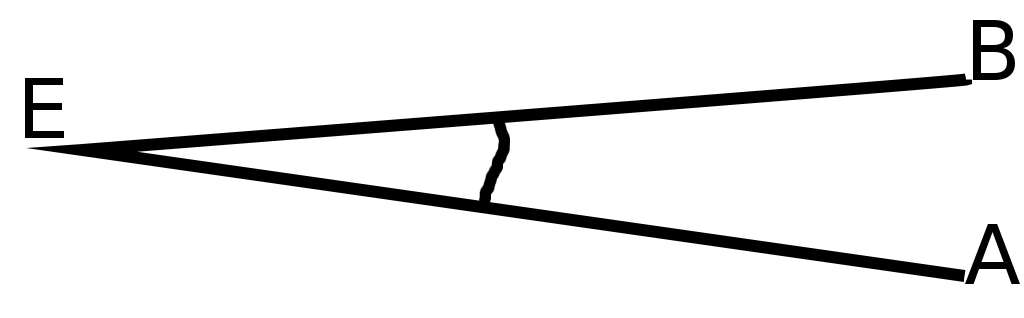
\includegraphics[height=1.5cm]{aeb.png}
					\end{center}

% 				\end{figure}
% 			\end{multicols}
		\end{fmerke}

		\begin{fmerke}[Winkel in $\mathbf{C}$]
			$\cos (\phi) = \frac{Re \langle x, y \rangle}{\parallel x \parallel \cdot \parallel y \parallel}$
		\end{fmerke}

	\subsection{Äusseres Produkt}
	
		\begin{fdef}[Äußeres Produkt]
			$xy^H = $ Matrix Rang 1
		\end{fdef}
		
		\begin{fsatz}[Orthogonale Projektion]
			Projektion $P_y(x)$ des Vektors $x$ auf Gerade $y$ durch Ursprung\\
			$P_y(x) = \frac{1}{{||y||}^2} \cdot yy^H x = uu^Hx$ wobei $u = \frac{y}{||y||}$\\
			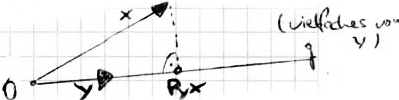
\includegraphics[width=7.2cm]{ortho_projektion} 
		\end{fsatz}

		\begin{fdef}[Householder-Spiegelung]
			Spiegelung an Hyper-spiegelebene (geg durch dazu orthogonalen Einheitsvektor $u$):\\[-5mm]
			\begin{floatingfigure}[p]{3.4cm}
				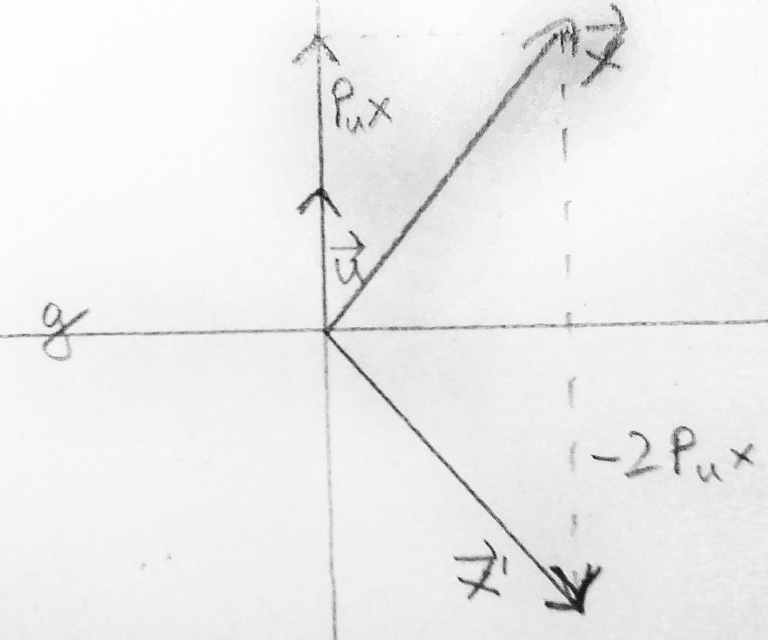
\includegraphics[width=3.3cm]{householder}
			\end{floatingfigure}
			$$H_u = I -  2 \cdot u u^H$$\\[-5mm]

			Ein Vektor wird durch $H_u x$ an der Hyperebene gespiegelt
			\vspace{8mm}
		\end{fdef}
		

		
	\subsection{Orthogonale / Unitäre Matrizen}
		
		\begin{fdef}[Orthogonal $\R$, unitär $\C$]
			$A^H\cdot A = I \quad \Rightarrow \quad A^{-1} = A^H$ 
		\end{fdef}
		
		\begin{feig}[Eigenschaften]
			$A$ unitär $\quad \leftrightarrow A^{-1} \quad$ unitär\\
			$A$ unitär, $B$ unitär $\quad \leftrightarrow \quad AB$ unitär\\[2mm]
			\textbf{Abbildungen mit A:}\\
			$||Ax|| = ||x||$ (längentreu)\\
			$\left< Ax, Ay \right> = \left< x,y \right>$ (winkeltreu)
		\end{feig}
%\end{multicols}

	
\section{Zerlegungen}
%\begin{multicols}{2}
	
	\vspace{-2mm}
	\subsection{LR-Zerlegung}
		
		\begin{falgo}[LR-Zerlegung]
			Wie Gauß-Algorithmus. Zusätzlich werden aber die Faktoren, die nötig waren um das Element an dieser Stelle zu 
			eliminieren, in einer Matrix $L$ gespeichert, wobei $l_{jj} = 1$. Der Faktor $f$ bedeutet dann, dass die Pivotzeile
			im Eliminationsschritt mit $f$ multipliziert und von der aktuellen Zeile \textit{subtrahiert} wird. \\

			Damit erhält man \vspace{-1mm} $$PA = LR$$\\[-6mm] wobei $P$ die Permutationsmatrix ist, die die Zeilenvertauschungen mitführt
		\end{falgo}
		
		Vorteil gegenüber Gauß: \\
		$b$ wird nicht verändert $\rightarrow$ austauschen $\rightarrow$ leicht $x$ neu berechnen
		
		\begin{fmerke}[LGS aus LR lösen]
			\vspace{-4mm}
			\begin{align*}
				\text{ Es sei } Ax & = b \\
				(P)A & = LR   &\rightarrow  L,R &\quad \\
				Ly   & = (P)b &\rightarrow  y &\quad \\
				Rx   & = y    &\rightarrow  x &\quad
			\end{align*}
			\vspace{-6mm}
		\end{fmerke}
		
		\begin{falgo}[Cholesky-Zerlegung]
			Berechne $\tilde R$ mit $A = \tilde R^H \tilde R$, $A$ muss spd (\textit{symmetrisch und positiv definit}) sein.
			$$r_{ij} = 
			\begin{cases}
			0 & \text{für}\ j < i\\
\sqrt{a_{ii} - \sum\limits_{k=1}^{i-1}|r_{ki}|^2 } & \mathrm{f\ddot{u}r}\ i = j\\
\frac{1}{r_{ii}} \left( a_{ij}-\sum\limits_{k=1}^{i-1}\overline{r_{ki}} r_{kj} \right) & \mathrm{f\ddot{u}r}\ j > i
\end{cases}$$\\[-6mm]
		\end{falgo}
			
		\begin{fmerke}[Anwendungen]
			\textbf{spd-Test} Wenn nicht spd, bricht Chol ab\\
			\textbf{LGS-lösen} schneller als LR, geht aber nur wenn spd
		\end{fmerke} 


%\end{multicols}
\section{Vektorräume}
%\begin{multicols}{2}

	\begin{fdef}[Vektorraum]
		Ein Körper, mit Vektoren als Elemente der Vektoraddition und der skalaren Multiplikation
	\end{fdef}
	
	\begin{feig}[Axiome des Vektorraumes]
		\renewcommand{\labelenumi}{(V\theenumi)}
		
		\begin{enumerate}
			\item $x + y = y + x$\\[-5.5mm]
			\item $(x + y) + z = x + (y + z)$\\[-5.5mm]
			\item es gibt ein Element $o \in V$ für das gilt $x + o = x$\\[-5.5mm]
			\item $\forall x \in V$  $\exists \, {-x} \in V$\\[-5.5mm]
			\item $\alpha(x + y) = \alpha{}x + \alpha{}y$\\[-5.5mm]
			\item $(\alpha + \beta)x = \alpha{}x + \beta{}x$\\[-5.5mm]
			\item $(\alpha{}\beta{})x = \alpha{}(\beta{}x)$\\[-5.5mm]
			\item $1x = x$
		\end{enumerate}
		\vspace{-2.5mm}
	\end{feig}
	
	\begin{fdef}[Unterraum]
		Eine nichtleere Teilmenge $U \subseteq V$ ist ein Unterraum, wenn $\forall x,y \in U \land \alpha \in \mathbb{E}$ gilt:
		\begin{align*}
			x+y \in U \\
			\alpha x \in U
		\end{align*}

	\end{fdef}
	\textbf{Beispiel:} $\mathcal{P}_0 \subset \mathcal{P}_n \subset \mathcal{P} \subset C^{\infty}(\R)
						\subset C^n(\R) \subset C^0(\R)$\\
	wobei $C^n$ alle mind. $n$ mal ableitbaren Funktionen und $\mathcal{P}_n$ die Polynome mit Maximalgrad $n$ sind
	
	\begin{fdef}[Erzeugendensystem]
		spannt einen Vektorraum auf\\
		$\text{span} \{a_1, a_2, \ldots, a_n \}$
	\end{fdef}

	\begin{fdef}[Basis]
		Lineareres unabhängiges Erzeugendensystem
	\end{fdef}
	
	\begin{fdef}[Linearkombination]
		Jeder Vektor x ist als Linearkombination darstellbar:\\
		$\beta_1 a_1 + \ldots + \beta_n a_n = x$
	\end{fdef}
	
	\begin{feig}[Linear unabhängig]
		Eine Menge von Vektoren ist linear unabhängig, wenn kein Vektor eine Linearkombination der Anderen ist, Test mit Gauss:\\
		$Ax = 0$ hat nur triviale Lös. $x=\overrightarrow{0}$
	\end{feig}

	
	\subsection{Basiswechsel}
	
		\begin{fdef}[Transformationsmatrix]
			führt den Wechsel zwischen zwei Basen $B$ und $B'$ durch. $\xi$ ist der Koordinatenvektor vom Vektor $x$
			bzgl. der Basis $B$\\
	
			Jeder Vektor in der neuen Basis lässt sich als Linearkombination der alten Basis schreiben:
			\begin{align*}
				b_k' &= \sum_{i=1}^n \tau_{ik} \cdot b_i \qquad \text{'wir setzen }T = (\tau_{ik})^n_{ik=1} \\
				B' &= B \cdot T \qquad \text{ $T$ Transformationsmatrix }
			\end{align*}
			
		\end{fdef}
		\hspace{-5mm}
		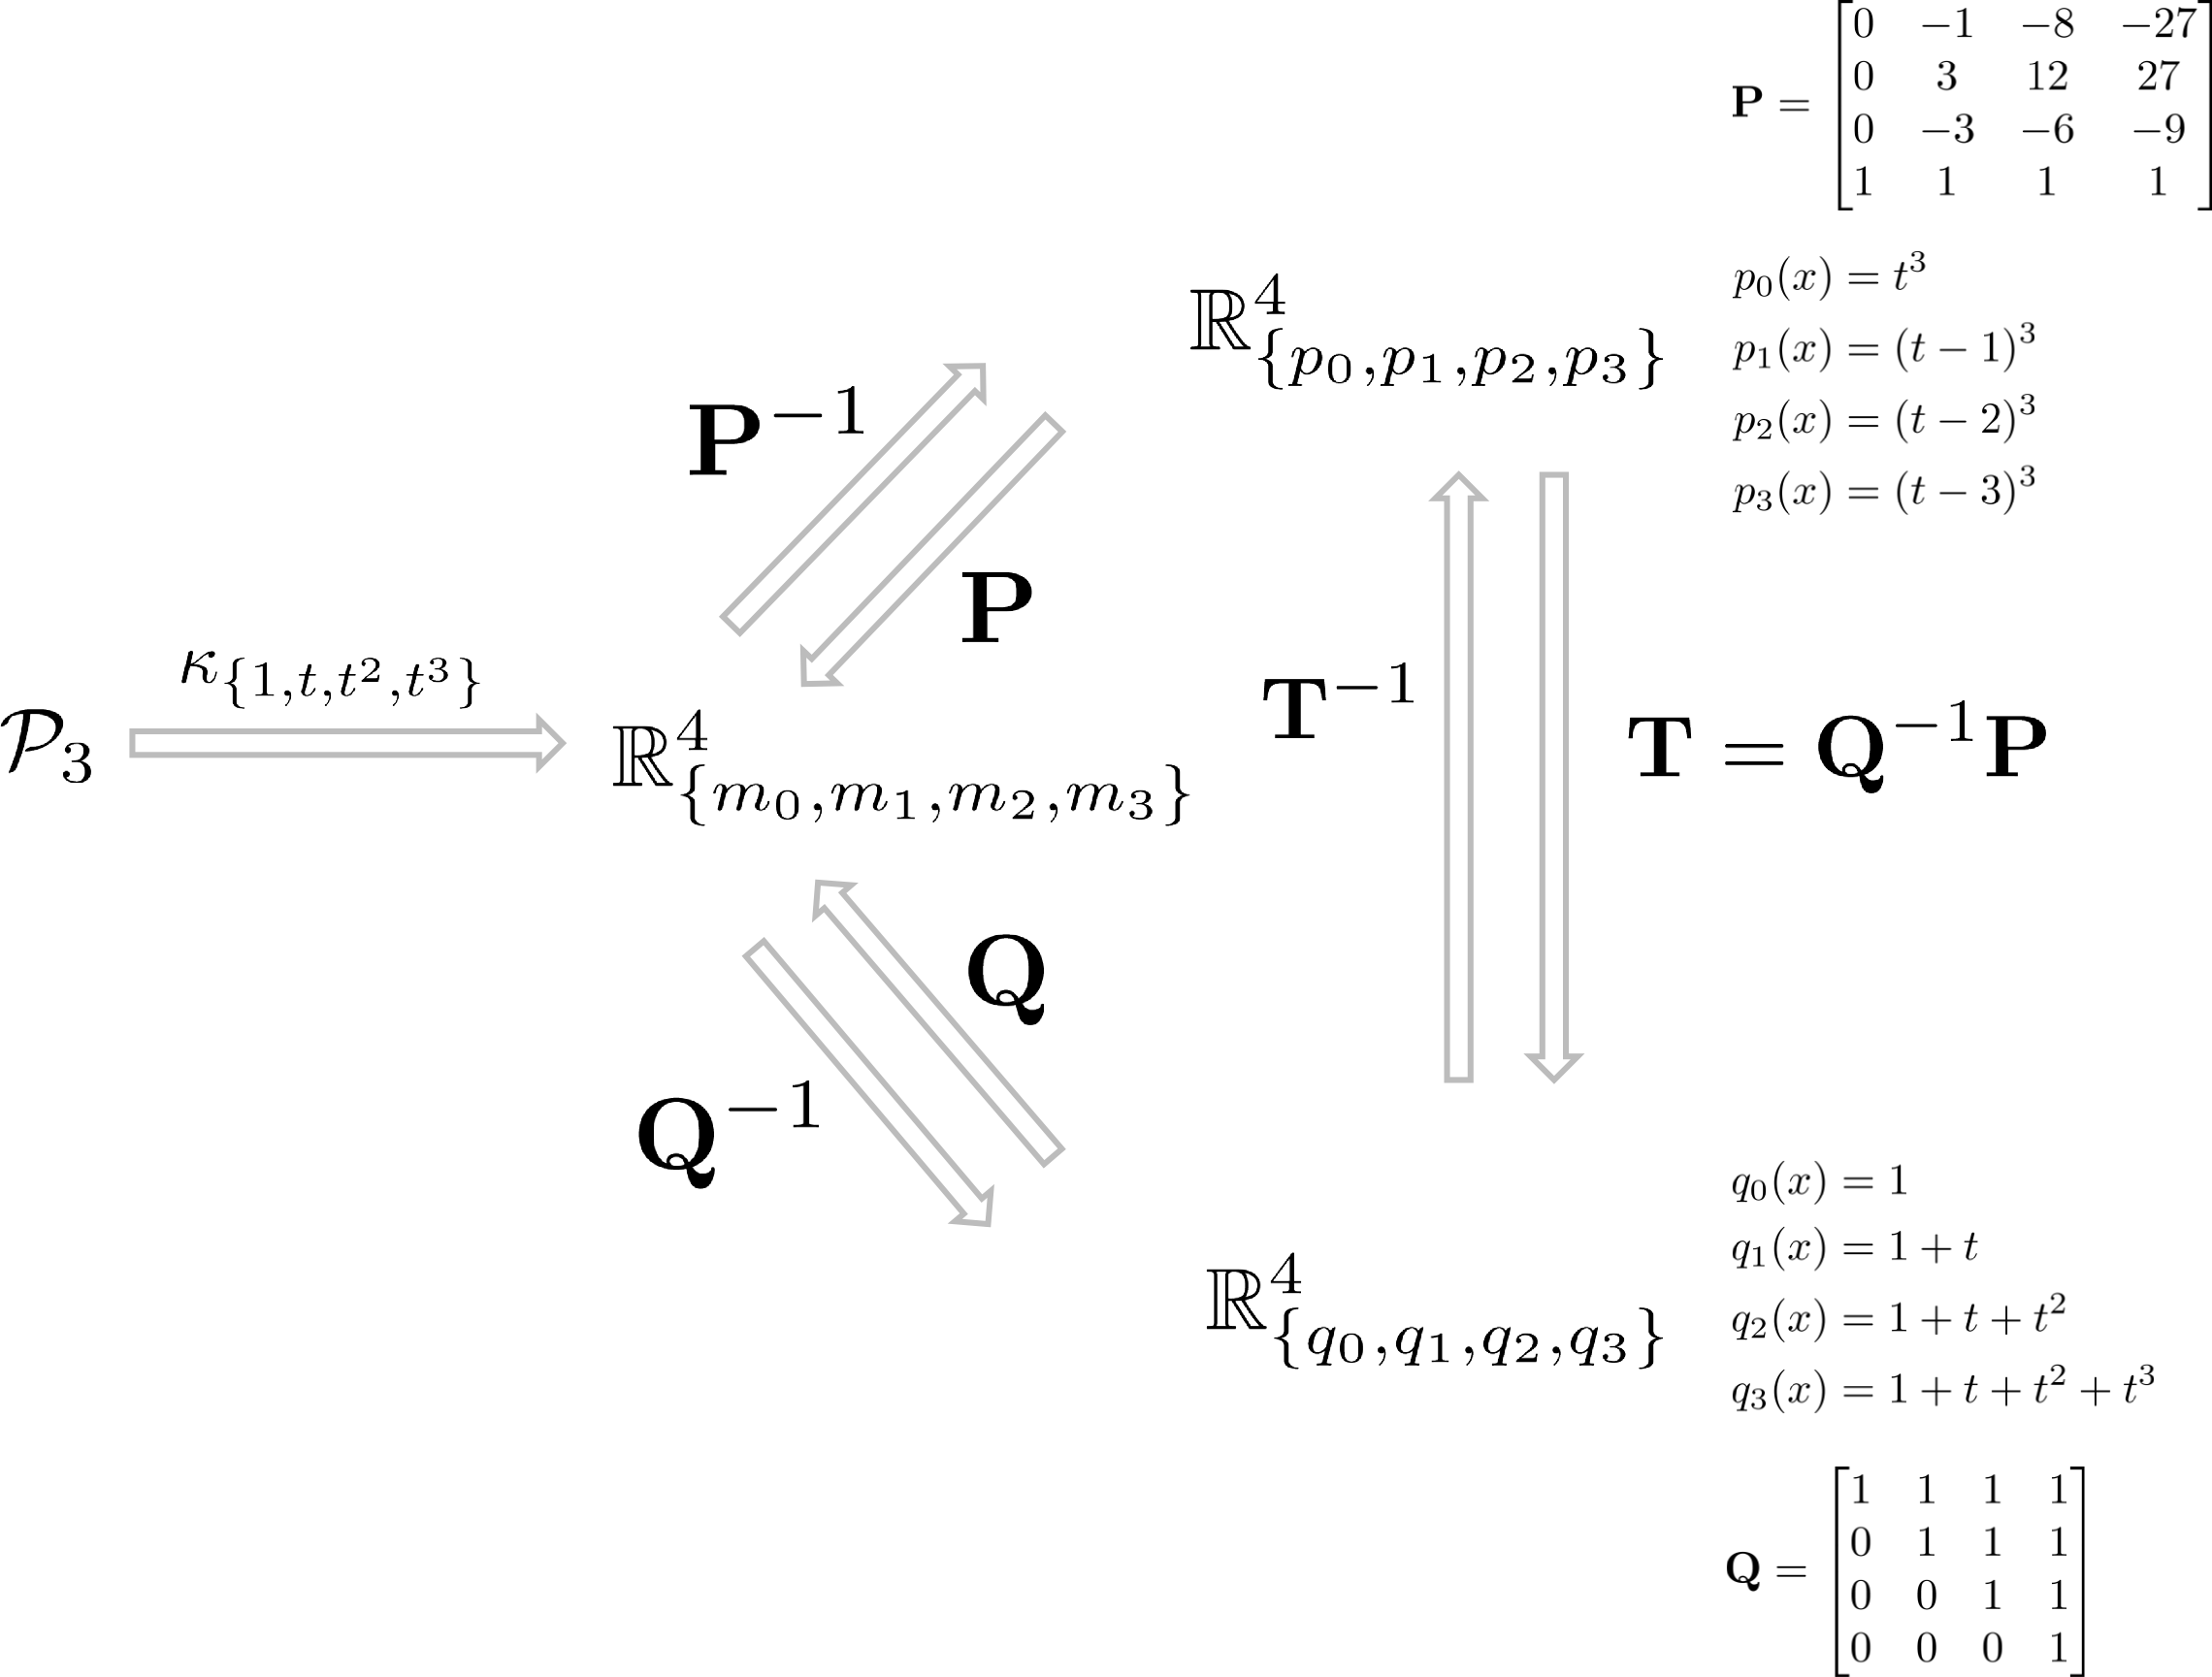
\includegraphics[width=10cm]{basistransformation_hoch.png}
		\begin{fregeln}[Formeln]
			$\xi ' = T^{-1} \cdot \xi$ \hspace{2mm} $\xi = T \cdot \xi '$\\
			$B' = B \cdot T$ \hspace{2mm} $B = B' \cdot T^{-1}$\\
			$B \cdot \xi = x = B' \cdot \xi '$
		\end{fregeln}
		
		\begin{fmerke}[$B$ = \textit{Standardbasis} $\mathbb{I}$]
			Ist $B$ \textit{Standardbasis}, also $\mathbb{I}$, so gilt:\\
			$B' = B \cdot T = \mathbb{I} \cdot T \rightarrow T = B'$\\[-4mm]
		\end{fmerke}
		
		\begin{fmerke}[Abb. A in \textit{sich}]
			Bei zwei Abbildungen $A$ und $C$:
			$C = T^{-1}AT$
		\end{fmerke}

		\begin{fmerke}
			\begin{center}
				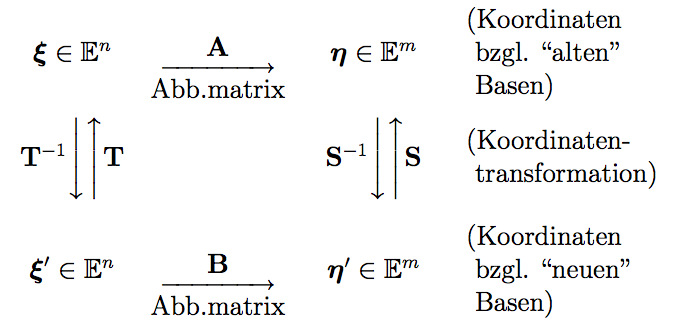
\includegraphics[width=8cm]{basiswechsel}
			\end{center}
			\vspace{-2mm}
		\end{fmerke}
%\end{multicols}
\section{Lineare Abbildungen}
%\begin{multicols}{2}

	\begin{fdef}[Abbildung]
		$F: X \to Y$ ist eine Abbildung
	\end{fdef}
	
	$X$ ist der Definitionsbereich $\text{dom}(F)$, $Y$ der Zielbereich $\text{range}(F)$ und die Menge der tatsächlich angenommenen Werte aus $Y$ heißt Wertebereich $\text{im}(F)$. 
	
		\begin{feig}[\begin{tabular*}{\textwidth}{@{\extracolsep{0mm}}l@{\extracolsep{\fill}}c@{\extracolsep{0mm}}r}injektiv & $\forall x_1, x_2 \in X : (f(x_1)= f(x_2)) \Rightarrow x_1=x_2$\end{tabular*}]
			Jedes Element Zielbereich \textbf{höchstens} einmal\\[-3.5mm]
		\end{feig}
	\begin{feig}[\begin{tabular*}{\textwidth}{@{\extracolsep{0mm}}l@{\extracolsep{\fill}}c@{\extracolsep{0mm}}r}surjektiv & $\forall y \in Y \ \exists x \in X : f(x)=y$\end{tabular*}]
			Jedes Element Zielbereich \textbf{mindestens} einmal
		\end{feig}
	\begin{feig}[bijektiv / isomorph]
		Jedes Element Zielbereich \textbf{genau} einmal, surjektiv und injektiv\\
		Ist eine Abbildung $F$ bijektiv, dann gibt es eine inverse Abbildung $F^{-1}$
	\end{feig}
	
	\begin{fmerke}[Zusammengesetzte Abbildungen]
		$G \circ F(x) = G(F(x)) = G \cdot F \cdot x$ 
	\end{fmerke}
	
	\begin{fdef}[Lineare Abbildung]
		Eine Abbildung ist linear, falls\\[-6mm]
		\begin{enumerate}
			\item $F(x + \tilde x) = F(x) + F(\tilde x)$\\[-6mm]
			\item $F(\alpha x) = \alpha F(x)$\\[-5mm]
		\end{enumerate}
		oder:
		$F(\beta x + \gamma \tilde x) = \beta F(x) + \gamma F(\tilde x)$
	\end{fdef}
	
	\begin{fdef}[Wichtige lineare Abb.]
		$C^n$ repräsentiert eine mind. $n$ mal ableitbare Funktion $f$ \\[-6mm]
		\begin{description}
			\item[Ableitungsoperator] $D:C^1 \rightarrow C$, $f \mapsto f'$\\[-6mm]
			\item[Differentialoperator] $L:C^m \rightarrow C$, $f \mapsto c_m f^{(m)} + c_{m-1} f^{(m-1)} + \cdots
										+ c_1 f' + c_0 f$
			\item[Evaluationsabb.] $t$ fest, $E_t:C \rightarrow \R$, $f \mapsto E_t f :\equiv f(t)$
			\item[Multi'op.] $M:C \rightarrow C$, $f \mapsto g$, wo $g(t) :\equiv t \cdot f(t)$
			\item[$\mathbf{F = M \circ D + E_2}$] $F:C^1 \rightarrow C$, $f \mapsto t f'(t) + f(2)$
		\end{description}
	\end{fdef}

	\begin{fdef}[Affine Abbildung]
		Eine affine Abbildung ist eine lineare Abbildung verknüpft mit einer Translation\\
		$H:X \rightarrow y_0 + Y$, $x \mapsto y_0 + Fx$ mit $F$ lineare Abb.
	\end{fdef}
	
	\subsection{Kern, Bild}
	
		\begin{fdef}[Kern]
			Die Menge der Vektoren $x \in \text{dom}(F)$ für die gilt: $Fx = 0$\\
			Mit $A$ lin. Abb., $ker A = \mathcal{N}(A) = $ Nullraum
		\end{fdef}
			\vspace{-3mm}
			$F$ injektiv $\leftrightarrow$ $\ker(F) = 0$
		
		\begin{fmerke}[Basis des Kerns von $A$]
			\begin{enumerate}
				\item Reduziere $A$ auf Zeilenstufenform
				\item löse $Ax = 0$
				\item Wähle in $x$ jeweils einen der freien Parameter $1$ und die anderen $0$. Die dadurch gewonnenen Vektoren $x_i$ sind die Basisvektoren des Kerns.
			\end{enumerate}
			\vspace{-3mm}
		\end{fmerke}
			
		\begin{fdef}[Bild]
			Menge der rechten Seiten $b$, für die $Ax=b$ eine Lösung hat 
			Mit $A$ lin. Abb., $im A = \mathcal{R}(A) = $ Kolonnenraum
		\end{fdef}

		\begin{fmerke}[Basis des Bildes von $A$]
			\begin{enumerate}
				\item Reduziere $A$ auf Zeilenstufenform
				\item Die Kolonnen, bei denen das Pivotelement $\ne 0$ ist, sind die Pivotkolonnen.
						Somit sind diese Kolonnen in der ursprünglichen Matrix $A$ Basisvektoren des
						Kolonnenraums, also des Bildes von $A$
			\end{enumerate}
			\vspace{-3mm}
		\end{fmerke}
		
		\begin{fsatz}[Dimensionsformel]
			$F : n \times m$-Matrix\\
			$\dim X = m = $ Anz. Basisvektoren \\
			$\dim \text{im } F = \text{Rang } F$ \\
			$\dim \ker F = $ Anz. freie Parameter\\[2mm]
			$\dim X - \dim \ker F = \dim \text{im } F$\\[2mm]
			oder auch, da $\dim \text{im } F = \text{Rang } F:$\\[1mm]
			\underline{$\dim X - \dim \ker F = \text{Rang } F$}
		\end{fsatz}
		
	\subsection{Orthonormalbasen}
		
		\begin{fdef}[Basis orthogonal]
			Alle Vektoren paarweise orthogonal
		\end{fdef}

		\begin{fdef}[Basis orthonormal]
			Alle Vektoren paarweise orthogonal und haben Länge $1$
		\end{fdef}
		
		\begin{falgo}[Gram-Schmidt Orthogonalisierung]
			$\mathbf{a_1, \ldots, a_n}$ linear unabhängige Vektoren (alte Basis)\\
			
			$
			\mathbf{b_{1}} := \frac{\mathbf{a_{1}}}{\|\mathbf{a_{1}}\|} \\
			\left. 	\begin{array}{rl}

				\mathbf{\tilde{b}_{k}} &:= \mathbf{a_{k}} - \sum_{j = 1}^{k -1} \langle \mathbf{b_{j}}, \mathbf{a_{k}} \rangle \cdot \mathbf{b_{j}} \\
				\mathbf{b_{k}} &:= \frac{\mathbf{\tilde{b}_{k}}}{\|\mathbf{\tilde{b}_{k}}\|}
					\end{array}
			\right\} (k = 2, \ldots, n)
			$
			
			$\mathbf{b_1, \ldots, b_n}$ paarweise orthonormale Vektoren (neue Basis)
		\end{falgo}
	\subsection{Normen von lin. Abb und Matrizen}
		
		\begin{fdef}[Matrixnorm]
			$$ \| . \|: \mathbf{E}^{n \times n} \rightarrow \mathbf{R}, \quad A \mapsto \| A \| = \sup_{x \neq 0} \frac{\| Ax \|}{\| x \|} = \sup_{\| x \| = 1} \| Ax \|$$
			\begin{description}
			\item[positiv definit] 
				\begin{align*}
					\| F \| \geq 0 \\
					\| F \| = 0 \Rightarrow F = 0
				\end{align*}
			\item[homogen]
				\begin{align*}
					\| \alpha F \| = |\alpha | \| F \|
				\end{align*}
			\item[Dreiecksungleichung]
				\begin{align*}
					\| F + G \| \leq \| F \| + \| G \|
				\end{align*}
			\item[zusammengesetzte Abbildungen]
				\begin{align*}
					\| F \circ G \| \leq \| G \| \| F \|
				\end{align*}
			\item[kompatibel mit den Vektornormen]
				\begin{align*}
					\| Fx \|_Y \leq \| F \| \| x \|_X
				\end{align*}
			\end{description}

		\end{fdef}
		
		\begin{fdef}[Spektralnorm]
			$$ \| A \|_2: \equiv \sup_{x \neq 0} \frac{\| Ax \|_2}{\| x \|_2} $$
			Bei einer Diagonalmatrix $D$ gilt:
			$$ \| D \|_2 = \max_{x \neq 0} \frac{\| Dx \|_2}{\| x \|_2} = \max_{1 \leq k \leq n} | d_{kk} |^2 = $$
			Daraus folgt:
			\begin{align*}
				\left\| A \right\|_2 &= \max \left\{ \sqrt{\omega}\text{; $\omega$ Eigenwert von $A^HA$}\right\}\\
						&= \max \left\{|\omega| \text{; $\omega$ Eigenwert von $A$}\right\}\\
				\left\| A^{-1} \right\|_2 &= \max \left\{ \frac{1}{| \omega |} \text{; $\omega$ Eigenwert von $A$}\right\}
			\end{align*}

		\end{fdef}
		
		\begin{fdef}[Frobeniusnorm]
			\begin{align*}
				\| A \|_F :\equiv \sqrt{\sum_{k=1}^n \sum_{l=1}^n | a_{kl} |^2}
			\end{align*}

		\end{fdef}
	\subsection{Konditionszahl}
		\begin{fdef}[Konditionszahl]
			$$\kappa( A ) = \| A \| \| A^{-1} \|$$
		\end{fdef}
		
		\begin{fdef}[2-Norm-Konditionszahl]
			\begin{align*}
				\kappa_2(A) &= \| A \|_2 \| A^{-1} \|_2 \\
							&= \frac{\sigma_1}{\sigma_n} \quad \left( \sigma_1=\max \{EW(A) \} \quad \sigma_n = \min \{ EW(A) \setminus 0 \} \right)
			\end{align*}
		\end{fdef}


%\end{multicols}
\section{Methode der kleinsten Quadrate}
%\begin{multicols}{2}
	Die Methoder der kleinsten Quadrate löst überbestimmte lineare Gleichungssysteme, welche im Allgemeinen keine Lösung haben. Wir
	wollen eine gute Näherung. Dazu minimieren wir die Länge des Residuenvektors des Gleichungssystems $A x = y$
	
	Dabei ist zu beachten, dass dabei eine Orthogonalprojektion auf die durch $A^H\cdot A$ aufgespannte Ebene ausgeführt wird.
	\begin{fdef}[Residuenvektor]
		$$r := y - Ax$$
		\vspace{-5mm}
	\end{fdef} 
	
	\begin{fdef}[Normalengleichung]
		Falls die Kolonnen von $A$ linear unabhängig sind, ist r minimal, wenn:
		$$x = (A^HA)^{-1}A^Hy$$\\[-9mm]
		$$\mathbf{A^HAx = A^Hy}$$
	\end{fdef}
	\vspace{-2mm}
		
	\subsection{QR-Zerlegung}
		\begin{falgo}[QR-Zerlegung]
			\textbf{1. $Q$ aus Gram-Schmidt}\\
				$Q := B_{\text{Gram-Schmidt}}$\\[1mm]
			\textbf{2. Rechtsdreiecksmatrix $R$ berechnen}\\
				$
				r_{11} := \|\mathbf{a_{1}}\| \\
				\left.
					\begin{array}{rl}
						r_{jk} &:= \langle \mathbf{b_j},\mathbf{a_k} \rangle \quad (j = 1, \ldots, k-1) \\
						r_{kk} &:= \|\mathbf{\tilde b_k}\|
					\end{array} 
				\right\} k = 2, \ldots, n
				$     
		\end{falgo}
	
	\begin{fmerke}[Lösung kleinste Quadrate mit QR]
		$$Rx = Q^Hy$$\\[-10mm]
	\end{fmerke}
	\begin{Huge}TODO\end{Huge}\\ Beispiel
	\begin{falgo}[Modifiziertes Gram-Schmidt-Verfahren mit Kolonnen-Pivot]
		Idee: vertauschen der Pivotkolonnen mit den Nullkolonne, wenn $Rang(A^{m \times n}) < n$\\
		\begin{align*}
			\begin{array}{l}
			q_1 = \frac{a_1}{||a_1||}	\\
			\tilde q_i = a_i - q_1 \langle q_1, a_i \rangle \quad (i = 2, \hdots , n)\\ \\
			\left.
				\begin{array}{l}
				\text{wähle $p \geq k$ mit $|| \tilde q_p || \neq 0$ und vertausche}\\
				\text{Kolonnen $p$ und $k$. berechne:}\\
					q_k = \frac{\tilde q_k}{|| \tilde q_k ||}\\
					\tilde q_i = \tilde q_i - q_k \langle q_k, \tilde q_i \rangle \quad (i = k+1,...,n) \\
					\text{ist } ||\tilde q_{k+1} || = \vdots = ||\tilde q_n|| = 0\\
					\text{so gilt $Rang(A) = k$ und man ist fertig}
				\end{array} \right\rbrace (k = 2,...,n)
			\end{array}
		\end{align*}

	\end{falgo}

%\end{multicols}
\section{Determinanten}
%\begin{multicols}{2}

	\begin{fdef}[Determinate]
		Zeigt an, ob ein Gleichungssystem eindeutig lösbar ist oder nicht
	\end{fdef}
	
	\begin{fsatz}[Regel von Sarrus]
		\textbf{$2 \times 2:$}\\[1mm]
		$\det{\left(\begin{array}{cc}a_{11} & a_{12} \\ a_{21} & a_{22}\end{array}\right)}
			= a_{11}a_{22} - a_{12}a_{21}$\\[.6mm]
			Merke: Fischregel!\\[2mm]
		\textbf{$3 \times 3:$}\\[1mm]
		$\det{\left(\begin{array}{ccc}
					a_{11} & a_{12} & a_{13} \\
					a_{21} & a_{22} & a_{23} \\
					a_{31} & a_{32} & a_{33}
				\end{array}\right)} \\ =
				a_{11} a_{22} a_{33} + a_{12} a_{23} a_{31} + a_{13} a_{21} a_{32} 
					- a_{13} a_{22} a_{31} - a_{11} a_{23} a_{32} - a_{12} a_{21} a_{33}$
	\end{fsatz}
	
	\begin{fsatz}[Determinante für $n \times n$-Matrix $A$]
		Es gilt: $\det{A} \ne 0 \Longleftrightarrow \text{Rang}A = n \Longleftrightarrow A \text{ ist regulär}$\\
		Für $\det{A}$ gilt, mit $v =$ Anz. durchgeführter Zeilenvertauschungen und $r_{kk} =$ Pivotelement
		der reduzierten Matrix $A$:
		$$\det{A} = (-1)^v \cdot \prod^n_{k=1} r_{kk}$$
	\end{fsatz}

	\begin{fsatz}[Entwicklung nach Zeilen und Kolonnen]
		\textbf{Untermatrix} $A_{[k,l]}$ zum Element $a_{kl}$ erhält man durch Streichen der Zeile $k$ und Kolonne $l$ von $A$.\\
		\textbf{Kofaktor} $\kappa_{kl} :\equiv (-1)^{k+l} \cdot \det{A_{[k,l]}}$\\[2mm]

		Nun gilt für jede $n \times n$-Matrix $A$ für jedes feste $k$ bzw. jedes feste $l$ die Formeln
		$$\det{A} = \sum^n_{i=1} a_{ki} \kappa_{ki} = \sum^m_{i=1} a_{il} \kappa_{il}$$
		
		Ein Beispiel für die Entwicklung nach der ersten Zeile ist der Laplacesche Entwichklungssatz (s. u.).
	\end{fsatz}

	\begin{fmerke}[Laplacescher Entwickungssatz, Beispiel]
		$\begin{vmatrix}
			0 & 1 & 2 \\
			3 & 2 & 1 \\
			1 & 1 & 0
		\end{vmatrix}
			=
		0 \cdot
		\begin{vmatrix}
			2 & 1 \\
			1 & 0
		\end{vmatrix}
			-1 \cdot
		\begin{vmatrix}
			3 & 1 \\
			1 & 0
		\end{vmatrix}
			+2 \cdot
		\begin{vmatrix}
			3 & 2 \\
			1 & 1
		\end{vmatrix}
			= 0 + 1 + 2
		= 3$\\[1mm]
		Für größere Matrizen einfach rekursiv anwenden!
	\end{fmerke}
	
	\begin{fmerke}[Determinante einer Dreiecksmatrix]
		Die Determinante einer Dreiecksmatrix ist gleich dem Produkt der Diagonalelemente
	\end{fmerke}

	\begin{fmerke}[Determinante einer Block-Dreiecksmatrix]
		Die Determinante einer Dreiecksmatrix ist gleich dem Produkt der Determinante der Diagonalblockmatrizen\\
		$\begin{vmatrix}
			A & B \\
			0 & D
		\end{vmatrix} = \det{A} \cdot \det{D}$ (Linksblocksdreiecksmatrix analog)
	\end{fmerke}

	\begin{feig}[Eigenschaften]
		\begin{itemize}
		\item $\det(I) = 1$\\[-6mm]
		\item $\det(AB) = \det(A) \cdot \det(B)$\\[-6mm]
		\item $\det(A^{-1}) = \det(A)^{-1}$\\[-6mm]
		\item Werden $k$ Zeilen (oder Spalten) mit $\alpha$ multipliziert, ergibt sich $\det(A') = \alpha^k \cdot \det(A)$\\[-6mm]
		\item $\det(\alpha A) = \alpha^n \cdot \det(A) $\\[-6mm]
		\item $\det(A^{H}) = \overline{\det(A)}$\\[-6mm]
		\item Nullzeile / Kolonne $\rightarrow$ $\det(A) = 0$\\[-6mm]
		\item $\det(A)$ unverändert, wenn man zu einer Zeile ein Vielfaches einer anderen Zeile addiert\\[-6mm]
		\item Rang(A) $< n \rightarrow \det = 0$\\[-6mm]
		\item Sind $A$ und $B$ ähnlich, d. h. existiert $X$, sd. $A = X^{-1}\cdot B\cdot X$, dann gilt: $\det A = \det B$\\[-6mm]
		\end{itemize}
	\end{feig}

	\begin{fsatz}[Cramer'sche Regel]
		Lösen eines LGS mit Determinanten\\
		$$x_i = \frac{\det(A_i)}{\det(A)}$$
		Die Matrix $A_i$ entsteht aus der Matrix $A$, indem man die $i$-te Spalte durch die rechte Seite des Gleichungssystems ersetzt.
	\end{fsatz}
%\end{multicols}
\section{Eigenwerte}
%\begin{multicols}{2}

	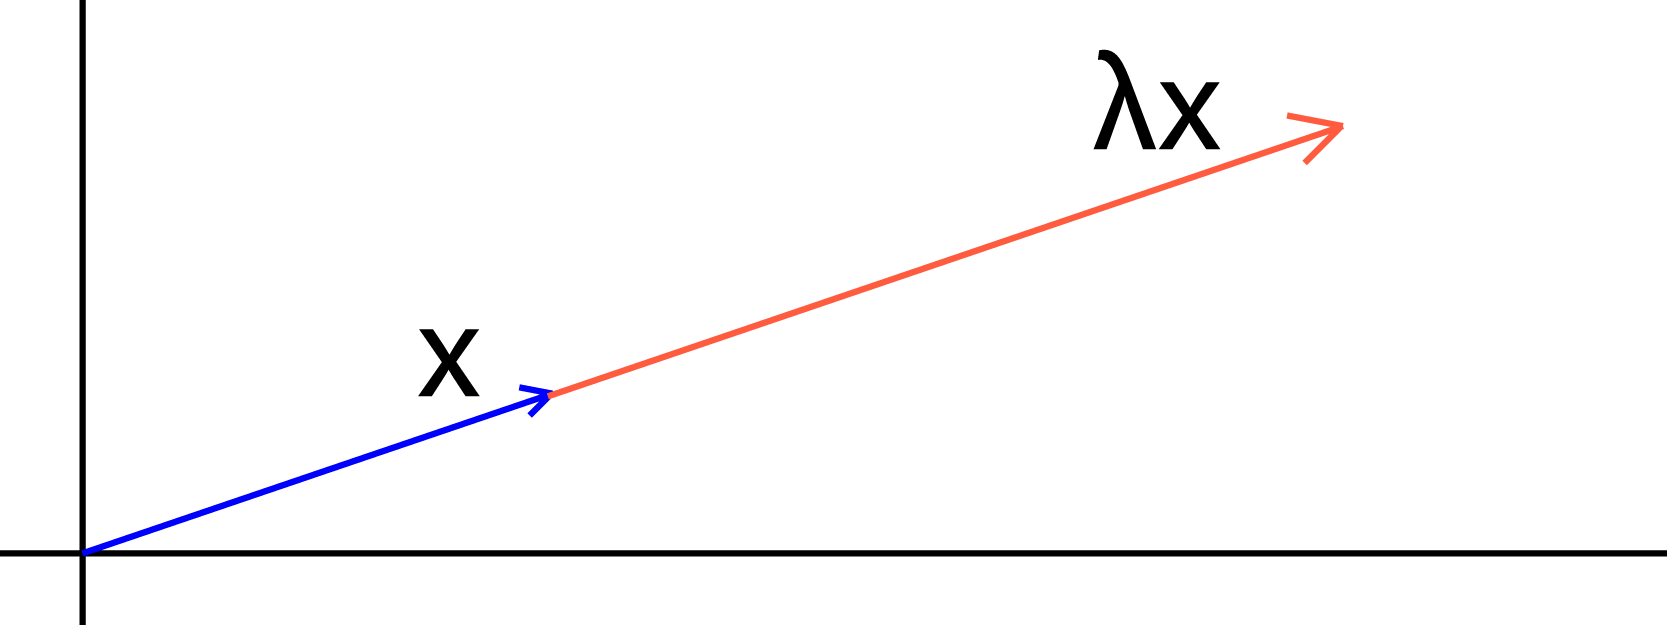
\includegraphics[width=6cm]{eigen}

	Betrachte die Abbildung $Ax = \lambda x$, $\lambda \in \C$
	
	\begin{fdef}[Eigenvektoren]
		$x$ ist Eigenvektor (\textbf{EV}) von $A$, wenn er durch Multiplikation mit $A$ nur um einen Wert $\lambda$ gestreckt wird.
	\end{fdef}
		\vspace{-3mm}
		Die Eigenvektoren einer Matrix sind linear unabhängig
		
	\begin{fdef}[Eigenwerte]
		$\lambda$ heißt Eigenwert (\textbf{EW}) der Abbildung $A$. Es ist der Wert, um den $x$ gestreckt wird
	\end{fdef}
	
	\begin{fmerke}[Eigenwerte sind Diagonalelemente]
		Sei $A$ eine $\triangle$-Matrix, so sind die EW die Diagonalelemente.
	\end{fmerke}

	\begin{fdef}[Spektrum]
		$\sigma(A) :\equiv$ Die Menge der Eigenwerte einer Matrix
	\end{fdef}

	\begin{fdef}[Eigenraum (ER)]
		Ist $\lambda$ EW, so ist der zugehörige Eigenraum $E_\lambda$ gleich der um den Nullvektor erweiterten
		Menge der EV zu $\lambda$:\\
		$E_\lambda :\equiv \{v \in V; Av = \lambda v\}$
	\end{fdef}
	
	\begin{fdef}[geom. Vielfachheit]
		Die geometrische Vielfachheit eines EW $\lambda$ ist gleich der Dimension von $E_\lambda$, also die Anz. EV von $\lambda$\\[1mm]
		$\dim E_\lambda = \dim(ker(A-\lambda I)) = n - \text{rang}(A - \lambda I)$
	\end{fdef}
	
	\begin{fdef}[algbr. Vielfachheit]
		Die algebraische Vielfachheit eines EW $\lambda$ ist die Vielfachheit von $\lambda$ als Nullstelle des char. Polynoms
	\end{fdef}
	$\forall$ EW: geom. Vielfachheit $\le$ algebr. Vielfachheit\\
	(geom. = algebr. Vielfachheit $\Leftrightarrow$ Matrix diagonalisierbar
	$\leftrightarrow$ Wenn $A$ lauter verschiedene EW hat, ist sie diagonalisierbar
	
	\begin{feig}[Eigenschaften falls A sym./herm.]
		\begin{itemize}
			\item Alle EW sind reell\\[-6mm]
			\item Kommen alle EV von verschiedenen EW, dann sind sie orthogonal\\[-6mm]
			\item Es existiert eine Eigenbasis (Basis aus EV), die orthogonal ist\\[-6mm]
			\item Für $U$ unitär gilt: $U^HAU = D = \text{diag}(\lambda_1, \ldots \lambda_n)$\\[-6mm]            
		\end{itemize}
	\end{feig}
			
	\begin{fmerke}[Berechnung der EV und EW]
		\textbf{1. Char. Polynom aufstellen}
			\vspace{-2mm}
			$$\chp(\lambda) = \det(A-\lambda I) = \chi_A$$ \\[-6mm]
		\textbf{2. Nullstellen (=Eigenwerte) bestimmten}\\[1mm]
		\textbf{3. Eigenvektoren berechnen}
			\vspace{-2.5mm}
			$$(A-\lambda_i I)v = 0 \text{  oder  } A v = \lambda v\text{ lösen}$$\\[-8mm]
			d. h. berechnen maximal vieler unabhängiger Lösungen durch Nullsetzen aller freien Parameter ausser einem, den wir
			auf 1 setzen (wiederholen für jeden Param.)%\\
%			Wenn algeb. Vielf. v. $\lambda \ne $ Anz. EV v. $\lambda$, berechne \textit{Hauptvektoren}
	\end{fmerke}
	
%	\begin{fdef}[Hauptvektor (HV), alg. Eigenraum]
%		EV sind HV 1. Stufe. Für HV $p$-ter Stufe gilt:
%		$$(A - \lambda E)^p\, v=0$$
%		Die Menge aller HV (und EV) spannen den alg. ER ($aER$) auf. Wobei gilt:
%		$$\dim aER = \text{algeb. Vielfachheit } (\lambda)$$
%		Somit ist die Anz. aller HV (inkl. EV) $= \dim aER$
%	\end{fdef}
%	
%	\begin{fmerke}[Berechnung der HV]
%		Wenn $n = \text{algeb. Vielf. } - \text{ Anz. EV} > 0$, dann gibt es noch $n$ weitere HV, die wie folgt berechnet
%		werden können:
%		$$(A - \lambda I) w_{k + 1} = w_{k}$$
%		wobei $w_{1}$ ein HV 1. Stufe ist, also ein EV
%	\end{fmerke}


	\begin{fdef}[Eigenbasis]
		Basis aus Eigenvektoren
	\end{fdef}

	\begin{feig}[A, B ähnlich]
		$A$ und $B$ heißen ähnlich, wenn 
			$$A = T B T^{-1}    \quad   B = T^{-1} A T$$
		$\rightarrow$ A,B: gleiche Spur, Det und Eigenwerte
	\end{feig}
	
		Zu $A$ gibt es eine ähnliche Diagonalmatrix $D$ gdw. $\exists$ Eigenbasis von $A$

	\begin{fsatz}[Eigenwertzerlegung (Spektralzerlegung)]
		Zu $A$ gibt es die ähnliche Diag.Matrix $\Lambda$ genau dann, wenn es eine Eigenbasis von $A$ gibt. Für diese Basis $V$ gilt:
		$$A V = V \Lambda \quad A = V \Lambda V^{-1}$$
		
		wobei $V$ eine Matrix mit den Eigenvektoren als Spalten und $\Lambda$ eine Matrix mit den Eigenwerten in der Diagonalen ist (kann evt. nicht funktionieren)\\[1mm]
		$A$ heißt diagonalisierbar, wenn $\Lambda$ eine Diagonalmatrix ist
	\end{fsatz}
	
		\begin{fdef}[Spur von $A$]
			Die Spur von $A$ ist gleich der Summe der Diagonalelemente von $A$
		\end{fdef}
	
	\begin{fmerke}[Spezialfall A ($n = 2,3$)]
		$n=2$: $\chp(\lambda) = \lambda^2 -(a_{11}+a_{22}) \lambda + \det(A)$\\
		$n=3$: $\chp(\lambda) = \lambda^3 - \operatorname{spur}(A)\cdot\lambda^2 +$\\[-4mm]
				$$\left( \det(A_1) + \det(A_2) + \det(A_3) \right)\cdot\lambda - \det(A)$$\\[-5mm]
		wobei $A_i$ die $2 \times 2$ - Matrix $A$ ohne die $i$-te Zeile und Spalte ist.
	\end{fmerke}
		
	
	
	\subsection{Funktionen von Matrizen}
	
		\begin{fdef}[Anwenden einer Funktion]
			\begin{align*}
				f(\Lambda) := \text{diag}(f(\lambda_1), \ldots, f(\lambda_n))\\
				f(\Lambda) := V f(\Lambda) V^{-1}
			\end{align*}
		\end{fdef}
		\begin{fmerke}[e-Funktion]
			\begin{align*}
				e^{A} = V\cdot e^{\Lambda} V^{-1} = V 
				\left(
				\begin{array}{cccc}
					e^{\lambda_1} & 0 			   & \cdots & 0 \\
					0			   & e^{\lambda_2} & \cdots & 0 \\
					\vdots		   & \cdots		   & \ddots & \vdots\\
					0			   & \cdots		   & 0	    & e^{\lambda_n}
				\end{array}
				\right)
				V^{-1}
			\end{align*}
		\end{fmerke}
	\subsection{Anwendungen der Eigenwertzerlegung}
%%%%%%%%%%%%%%%%%%%%%%%%%%%%%%%%%%%%%%%%%%%%%%%%%%%%%%%%%%%%%%%%%%%%%%%%%%%%%%%%%%%%%%%%%%%%%%
		\begin{fmerke}[Schema für homogene, lineare Differentialgleichungen]
			Gegeben ist ein System erster Ordnung:
			\begin{align*}
				y_1'(t) &= a_{11}y_1(t)+a_{12}y_2(t)+...+a_{1n}y_n(t) \\
				y_2'(t) &= a_{21}y_1(t)+a_{22}y_2(t)+...+a_{2n}y_n(t) \\
						&\vdots \\
				y_n'(t) &= a_{n1}y_1(t)+a_{n2}y_2(t)+...+a_{nn}y_n(t) 
			\end{align*}
			Anfangsbedingungen:
			\begin{align*}
				y_1(0)=x_1 \quad y_2(0)=x_2 \quad \cdots \quad y_n(0)=x_n
			\end{align*}
			Schreibe das System um:
			\begin{align*}
				y'(t)=Ay(t)
			\end{align*}
			und erstelle die Eigenwertzerlegung von $A=V\Lambda V$
			\begin{align*}
				\underbrace{V^{-1}y'(t)}_{z'(t)}=\underbrace{V^{-1}AV}_{\Lambda} \underbrace{V^{-1}y(t)}_{z(t)}
				\xrightarrow{subst.} z'(t) = \Lambda z(t) 
			\end{align*}
			Das durch Substitution entstandene System $z'(t)=\Lambda z(t)$ hat nun die allgemeine Lösung:
			\begin{align*}
				\left. 
				\begin{array}{rl}
				z_1(t) &= \gamma_1 e^{\lambda_1 t}\\
					&\vdots	\\
				z_2(t) &= \gamma_2 e^{\lambda_n t}
				\end{array} 
				\right\rbrace 
				\Longleftrightarrow z(t) = e^{t\Lambda} \cdot
				\left( 
					\begin{array}{c}
						\gamma_1\\
						\vdots \\ 
						\gamma_n 
					\end{array} 
				\right)
				\Longleftrightarrow z(t) = c\cdot e^{t\Lambda}
			\end{align*}
			Die allgemeine Lösung lautet nun:
			\begin{align*}
				y(t) = Vz(t)=Ve^{t\Lambda}c
			\end{align*}
			
		\end{fmerke}
%\end{multicols}
%%%%%%%%%%%%%%%%%%%%%%%%%%%%%%%%%%%%%%%%%%%%%%%%%%%%%%%%%%%%%%%%%%%%%%%%%%%%%%%%%%%%%%%%%%%%%%
\section{Singulärwertzerlegung}
%	\begin{multicols}{2}
		\begin{fsatz}
			Sei A eine ``hohe'' $m \times n$ Matrix. mit $m \geqslant n$ und $Rang(A) = n$. So ist die Matrix $A^T \cdot A$  symmetrisch, positiv definit und invertierbar. So lässt sich in $A^TA$ in Eigenvektoren und Eigenwerte zerlegen: 
			\begin{align*}
				A^TA = V\Lambda V^T \\
				\text{wobei }\Lambda = \Sigma \cdot \Sigma = \Sigma^2 \text{ da }\Sigma \text{ Diagnoalmatrix } \Sigma = \sqrt{\Lambda}\\
				A^T\cdot A = V \Sigma \Sigma V \\
				\text{umgeformt...}\\
				\underbrace{(A \cdot V \cdot \Sigma^{-1})^T}_{U_1^T}  \cdot \underbrace{(A \cdot V \cdot \Sigma^{-1})}_{U_1}=I \\
				U_1 = A V \Sigma^{-1} \text{ ist eine orthogonale }m \times n\text{ Matrix.}
			\end{align*}
			Die Singulärwertzerlegung der Matrix $A$ ist nun folgendermassen definiert:
			$$A \cdot V \cdot \Sigma^{-1} = U_1\Rightarrow AV= U_1 \cdot \Sigma$$ $$\mathbf{A = U_1 \cdot \Sigma \cdot V^T}$$
			$U_1 = A \cdot V \cdot \Sigma^{-1}$\\
			$V$: Eigenvektoren von $A^T\cdot A$\\
			$\Sigma = \sqrt{\Lambda}$: Eigenwerte von $A^T \cdot A$ 
		\end{fsatz}
		
		\begin{fdef}
			$U$ = Eigenvektoren von $A\cdot A^T$\\(Orthonormale Basis im Spaltenraum von A)\\
			$V$ = Eigenvektoren von $A^T \cdot A$\\(Orthonormale Basis im Zeilenraum von A\\
		\end{fdef}
		
		\begin{fmerke}[Matlab]
			Eigenwerte und Eigenvektoren
			\begin{verbatim*}
				[U,V]=eig(A) 
			\end{verbatim*}
				Singulärwertzerlegung
			\begin{verbatim*}
				[S,V,D]=svd(A)
			\end{verbatim*}
		\end{fmerke}

		






%\end{multicols}
%%%%%%%%%%%%%%%%%%%%%%%%%%%%%%%%%%%%%%%%%%%%%%%%%%%%%%%%%%%%%%%%%%%%%%%%%%%%%%%%%%%%%%%%%%%%%%%
\section{Endliche Arithmetik}
%\begin{multicols}{2}

	\begin{fdef}[IEEE Floating Point Standard]
		\textbf{Single Precision (32Bit)}\\
			$\stackrel{S}{\overbrace{0}} \quad \stackrel{e}{\overbrace{1 \; \ldots \; 8}} \quad \stackrel{m}{\overbrace{9 \; \ldots \; 31}}$\\[2mm]
		\textbf{Double Precision (64 Bit)}\\
			$\stackrel{S}{\overbrace{0}} \quad \stackrel{e}{\overbrace{1 \; \ldots \; 11}} \quad \stackrel{m}{\overbrace{12 \; \ldots \; 63}}$
	\end{fdef}
	
	\begin{fmerke}[Umwandlung IEEE $\leftrightarrow$ Dez]
		Single: $a = (-1)^S \cdot 2^{e-127} \cdot 1,m$\\
		Double: $a = (-1)^S \cdot 2^{e-1023} \cdot 1,m$\\[1mm]
		Bsp: $m = 010010 \ldots 0 = 0 + \frac{1}{4} + 0 + 0 + \frac{1}{32} + \ldots + 0$ 
	\end{fmerke}
		
	\begin{fmerke}[Umwandlung Dez $\leftrightarrow$ IEEE]
		Bsp 30,4
		\begin{tabular}{cccccccccccccccccccccc}
			30 & $\rightarrow$ & /2 & 15 & $\rightarrow$ & -1 & $\rightarrow$ & /2 & $\rightarrow$ & 7 & $\rightarrow$ & -1 & $\rightarrow$ & /2 & $\rightarrow$ & 3 & $\rightarrow$ & -1 & $\rightarrow$ & /2 & $\rightarrow$ & 1\\
			$\downarrow$ &  &  & $\downarrow$ &  &  &  &  &  & $\downarrow$ &  &  &  &  &  & $\downarrow$ &  &  &  &  &  & $\downarrow$\\
			gerade &  &  & ungerade &  &  &  &  &  & ungerade &  &  &  &  &  & ungerade &  &  &  &  &  & ungerade\\
			$\downarrow$ &  &  & $\downarrow$ &  &  &  &  &  & $\downarrow$ &  &  &  &  &  & $\downarrow$ &  &  &  &  &  & $\downarrow$\\
			0 &  &  & 1 &  &  &  &  &  & 1 &  &  &  &  &  & 1 &  &  &  &  &  & 1
		\end{tabular}
		\begin{tabular}{ccccccccccccccccccccc}
			0.4 & $\rightarrow$ & *2 & $\rightarrow$ & 0.8 & $\rightarrow$ & *2 & $\rightarrow$ & 1.6 & $\rightarrow$ & -1 & $\rightarrow$ & *2 & $\rightarrow$ & 1.2 & $\rightarrow$ & -1 & $\rightarrow$ & *2 & $\rightarrow$ & 0.4\\
			$\downarrow$ &  &  &  & $\downarrow$ &  &  &  & $\downarrow$ &  &  &  &  &  & $\downarrow$ &  &  &  &  &  & \\
			$<$1 &  &  &  & $<$1 &  &  &  & $\geq$ 1 &  &  &  &  &  & $\geq$ 1 &  &  &  &  &  & \\
			$\downarrow$ &  &  &  & $\downarrow$ &  &  &  & $\downarrow$ &  &  &  &  &  & $\downarrow$ &  &  &  &  &  & \\
			0 &  &  &  & 0 &  &  &  & 1 &  &  &  &  &  & 1 &  &  &  &  &  & 
		\end{tabular}
	\end{fmerke}
	
	\begin{fmerke}[Ausnahmen]
		\renewcommand{\arraystretch}{1.5}
		\begin{tabular}{l || c | c}
						&   $m = 0$      &   $m \ne 0$\\\hline\hline
			$e = 255$   &   $\pm$ INF    &   NaN (Not A Number) \\\hline
			$e = 0$     &   Zahl $0$     &   $a = (-1)^S \cdot 2^{- \mathbf{126}} \cdot 0,m$\\
						&                &   $\uparrow$ \textbf{Denormalisierte Zahlen}
		\end{tabular}
	\end{fmerke}
	
	\begin{fdef}[normalisiert]
		$m = 1, \ldots$
	\end{fdef}
	
	\begin{fdef}[Maschinengenauigkeit]
		Kleinste Zahl $\epsilon$ für die gilt $\epsilon + 1 \ne 1$\\
		Single: $2^{-24}$, Double: $2^{-53}$
	\end{fdef}
	
	\begin{fmerke}
		$m := $ kleinste normalisierte positive Maschinenzahl\\
		$\overline{m} := $ kleinste denormalisierte positive Maschinenzahl\\[1mm]
		$m \cdot \epsilon = \overline{m}$
	\end{fmerke}
	
	\begin{fdef}[Absoluter / relativer Fehler]
		$e_{abs} = |\hat c - c|$\\
		$e_{rel} = \frac{e_{abs}}{|c|}$
	\end{fdef}
	
	\begin{fdef}[Auslöschung]
		Bei Subtraktion fast gleich grosser Zahlen wird das Ergebnis falsch. Bsp. 4-stellige Arithmetik: $\pi - 3.141 = 5.927 \cdot 10^{-4} \simeq 3.142 - 3.141 = 1.00 \cdot 10^{-3}$
	\end{fdef}
	
	\begin{falgo}[Kahan-Summation]
		Mit Hilfe von Kahan kann man den Summationsfehler minimieren. Die Summe $s_n = \sum_{j=1}^n x_j$ berechnet
		sich wie folgt, wobei $\ominus$ und $\oplus$ fehlerbehaftete $+$ und $-$ darstellen.\\
		\textbf{Intitialisierung:} $s_1 := x_1$, $c_1 := 0$\\[-3mm]
		$$\left.
		\begin{array}{l}
			Y   = x_j     \ominus c_{j-1} 	\\
			T   = s_{j-1} \oplus Y 			\\
			c_j = (T \ominus s_{j-1}) \ominus Y\\
			s_j = T  
		\end{array} 
		\right\} \text{Für } j = 2, \ldots , n
		$$
	\end{falgo}

%\end{multicols}
\section{Appendix}
%\begin{multicols}{2}
\begin{appendix}
	\begin{fmerke}[Horner-Schema]
		\textbf{Idee:} Algorithmus zur Auswertung eines Polynoms\\[-3mm]
		
		Beispiel: $x^3+4x+6$ an Stelle $x = 2$ lässt sich auch schreiben als $(((\mathbf{1}) \cdot x + \mathbf{0}) \cdot x + \mathbf{4}) \cdot x + \mathbf{6}$
		\begin{center}
			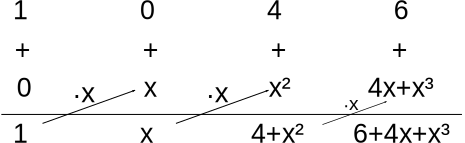
\includegraphics[width=6cm]{horner-schema}
		\end{center}
		Ergebnis: 22
	\end{fmerke}

	\begin{fmerke}[Reguläre Matizen]
		Ist $A$ regulär, dann sind folgende Aussagen äquivalent:\\[-6mm]
		\begin{itemize}
			\item $A$ hat vollen Rang\\[-6mm]
			\item $\det(A) \neq$ 0\\[-6mm]
			\item $A$ ist invertierbar\\[-6mm]
			\item Alle Zeilen- / Spaltenvektoren linear unabhängig\\[-6mm]
			\item 0 ist kein Eigenwert von A\\[-6mm]
			\item $\ker(A) = 0$\\[-6mm]
			\item$Ax = b$ besitzt genau eine Lösung\\[-6mm]
		\end{itemize}
	\end{fmerke}
	
	\begin{fmerke}[Matrix-Exponentialfunktion]
		$e^A = I + \frac{A}{1} + \frac{A^2}{2!} + \frac{A^3}{3!} + \ldots$\\
		$e^A = Ve^DV^{-1}$ falls $A$ diagonalisierbar
	\end{fmerke}
	
\section{Matlab}

	\renewcommand{\arraystretch}{1.2}
	\begin{tabular}{l | l}
		Maschinengenauigkeit    &   eps \\
		Transponieren           &   $A^T \rightarrow A'$\\
		Bereich                 &   $x =$ Anfang: Schritt: Ende \\
		Betrag                  &   abs(x)\\
		LR-Zerlegung            &   $A = LU$, [L,U,P] = lu(A)\\
		Cholesky-Zerlegung      &   $A = R^T \cdot R$, R = chol(A)\\
		EW-Zerlegung            &   [V,D] = eig(A)\\
		Determinante            &   det(A)
	\end{tabular}
	
	\vspace{3mm}

	\renewcommand{\arraystretch}{1.2}
	\begin{tabular}{l | l}
		ones(n)             &   $n \times n$ Matrix mit lauter 1en\\
		zeros(n)            &   $n \times n$ Matrix mit lauter 0en\\
		eye(n)              &   $n \times n$ Einheitsmatrix\\
		abs(a)				&	$|a|$, elementweise bei Matrix\\
		$[m,n]$ = size(A)   &   Größe einer Matrix\\
		norm(x)             &   Vektornorm\\
		norm(x,p)			&	$p$-Norm\\
		norm(x,inf)			&	$\infty$-Norm\\
		tril(A)/triu(A)     &   Unteres/oberes Dreieck (inkl. Diag.)\\
		A\^\;-1 = inv(A)    &   Inverses von A\\
		$x = A \backslash b$  & L"osung von $Ax=b$ \\
		diag(A) & Diagonale von A \\
		sum(diag(A))	&	Spur von A \\
		v=linspace(a,b,n)	&	$\leftrightarrow a:\frac{a-b}{n}:b$\\
		axis([a,b,c,d])		&	Setze X- und Y-Achsen manuell\\
		hold on bzw. off	&	Hält den aktuellen Plot\\
		plot(x,y)			& 	z.B. plot(cosx,sinx)\\
		polar($\phi$, $r(\phi)$)&Plottet $\phi$ gegen $r(\phi)$\\
		pol2cart($\phi$, r) &	Wandelt Polar in Kart. Koord.\\
		cart2sph(x,y,z)		&	Kart. nach Kugelkoord.
	\end{tabular}
	
	\begin{fdef}[Achtung!]
		Semicolon nicht vergessen
	\end{fdef}

\subsection{Syntax}
	\begin{tabular}{c|l}
		Operatoren										&		Bedeutung		\tabularnewline
		\hline
		$.+$, $.-$, $.*$, $./$, .\textasciicircum{} 	& 	Elementweise Operatoren \tabularnewline
		$+, -, *, /,$ \textasciicircum{} 				& 	Matrizen Addition, Multipl., etc. \tabularnewline
		$A'$											& 	$A^{H}$\tabularnewline
		$>, <, <=, >=, \sim =, ==$ 						& 	Vergleichsoperatoren\tabularnewline
		\&\&, $||$										& 	Boolsche Operatoren\tabularnewline
	\end{tabular}

	\begin{fmerke}
		\begin{verbatim}
			for i=1:5
			end
			
			while (a < A)
			end
	
			if (x == 1)
			elseif (x == 2)
			else
			end
			
			function [a,b] = name(arg1, arg2)
				return;       % optional
			end        % optional
			
			function summe=test1(A)
			[m,n]=size(A);
			summe=0;      % Initialisierung
			for i=1:m       % i geht von 1 bis m (Zeile)
				for j=1:n      % j geht von 1 bis n (Spalte)
				summe=summe+A(i,j);
				end
			end
		\end{verbatim}
		
	\end{fmerke}
	
	
		
\end{appendix}
%\end{multicols}
\end{document}
